% Generado desde README.md. Editar libremente.

\section{Contexto del proyecto}

\textbf{Qué es Poke Fresh.} Es un local de poke bowls (cuencos de arroz con pescado o pollo, salsas y toppings) que vende por la web. La persona arma su bowl o elige una promoción, paga en línea y lo retira en el local o, si vive a menos de 3 km, se lo llevan gratis. Dentro del local, cocina ve los pedidos pagados en el orden en que llegan y quien despacha asigna un chofer y registra la entrega. El dueño y el administrador mantienen productos, clientes y usuarios, y revisan las ventas.


\textbf{Qué pide el caso y qué pide esta evaluación.} El caso (requisitos R1 a R14, sección 0) ya tenía su frontend, que guardaba todo en el navegador. Esta evaluación pide lo que faltaba para que funcione de verdad: un backend con datos que se guardan, reglas de negocio, usuarios con permisos distintos, pagos con un proveedor externo y protección de los datos personales, todo conectado a las mismas pantallas.


\textbf{Qué tan grande es.} Es un solo local. Se estiman unos 150 pedidos al día (hasta 250 un viernes), unos 40 por hora en el almuerzo, es decir, unas 5 peticiones por segundo en el momento de más movimiento (es una proyección; la cuenta está en el ADR 0001). El sistema es pequeño en carga y delicado en datos, porque maneja RUN, direcciones y pagos. Por eso el diseño pone el esfuerzo en la seguridad y la claridad, no en escalar: la prueba de carga midió entre 209 y 316 peticiones por segundo, muy por encima de lo que el local necesita.


\textbf{La arquitectura, en un párrafo.} El navegador solo habla con una puerta, el API Gateway, que revisa quién es la persona y qué puede hacer, y recién entonces pasa la petición a un servicio privado (inventario, clientes, pedidos, pagos, autenticación o GraphQL). Los servicios no tienen puertos hacia afuera, cada uno guarda sus datos en su propia base de MongoDB y lee sus secretos de Vault. El pago ocurre en la página de una pasarela externa (aquí simulada), que después avisa al sistema con una notificación firmada.


\begin{figure}[H]
\centering
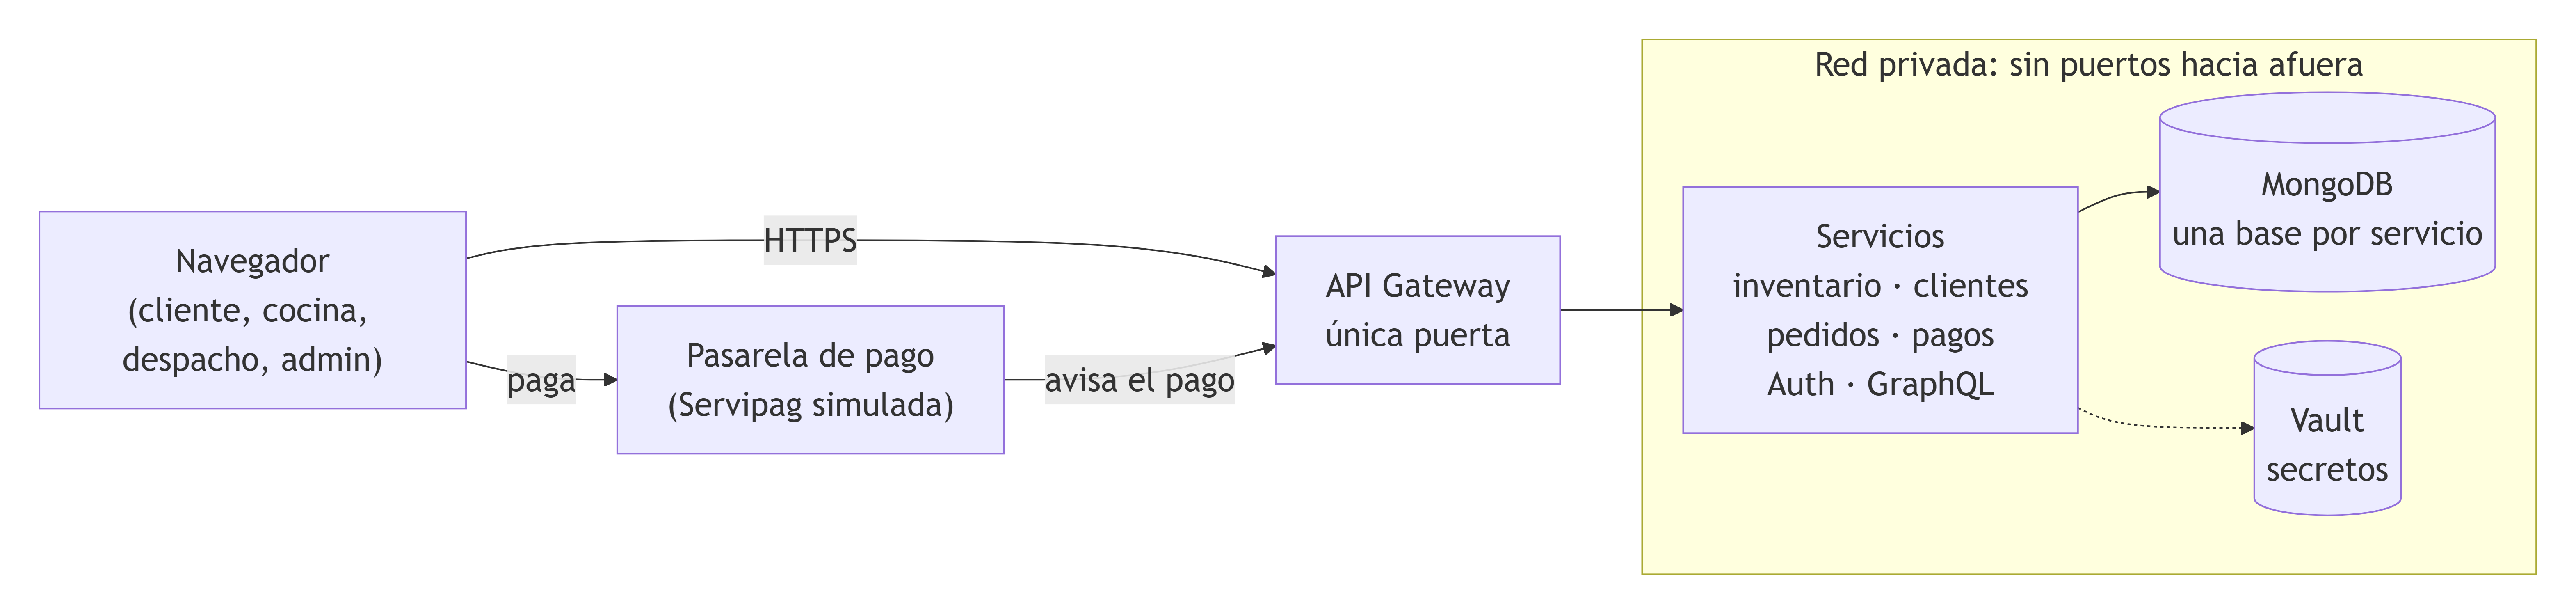
\includegraphics[width=\linewidth,height=0.85\textheight,keepaspectratio]{../diagramas/arquitectura-simple.png}
\caption{Arquitectura en una figura: el navegador entra por el API Gateway; los servicios, MongoDB y Vault están en una red privada}
\end{figure}

\textbf{Las decisiones que definen el diseño.}


\begin{enumerate}[nosep,leftmargin=*]
\item \textbf{Una sola puerta y servicios privados.} Lo que no se publica no se puede atacar. El gateway tiene una lista explícita de rutas permitidas; lo que no está en la lista no existe hacia afuera.
\item \textbf{Decide el servidor, no el navegador.} El navegador manda lo que la persona eligió; el precio, el total y si un pedido está pagado los calcula y decide el servidor. Un precio o un pago alterado desde la pantalla no tiene ningún efecto.
\item \textbf{Cada dato tiene un dueño y cada servicio tiene su propia llave.} Inventario decide los precios, pedidos decide el estado de un pedido, pagos decide el estado de un pago. Cada servicio usa su propia credencial, guardada en Vault, y todos los saltos van cifrados con TLS. Si se filtra una llave, solo abre una puerta.
\item \textbf{Lo simple primero.} Los servicios hablan REST; GraphQL se usa solo para juntar lecturas de varios servicios en una pantalla; no hay gRPC ni servicio de analítica aparte porque la carga medida no lo justifica (sección 9).
\end{enumerate}

\textbf{Una compra, de punta a punta.} Javiera Morales Díaz es la clienta de prueba que aparece en las capturas. Su compra recorre casi todo el sistema, y entre paréntesis va el número de cada operación (sección 1):


\begin{enumerate}[nosep,leftmargin=*]
\item Entra a la tienda y mira el menú: el navegador pide el catálogo y las reglas de armado (S01 y S03). No necesita sesión.
\item Ingresa con su correo y su clave (S33). El Auth Service valida la contraseña y el gateway le entrega una cookie que el JavaScript de la página no puede leer.
\item Arma un bowl regular de quinoa, salmón, salsa de goma, mango y edamame, y confirma el pedido (S15). El navegador manda solo qué eligió; inventario calcula el precio (\$6.990) y reserva los ingredientes.
\item Paga (S27). El sistema crea el cobro en la pasarela y la lleva a su página; Javiera paga allí y ningún dato de tarjeta pasa por Poke Fresh.
\item La pasarela avisa con una notificación firmada (S29). Si la firma, el monto y el cobro coinciden, pedidos marca el pedido como pagado, registra la venta y emite la boleta (la N° 79 en las capturas). El aviso a cocina y el correo con la boleta salen por una cola de mensajes, sin demorar el pago.
\item Cocina ve el pedido en su cola (S16), lo acepta (S20) y lo marca listo (S21). Javiera retira en el local, así que queda “listo para retiro”; si hubiera pedido despacho, el encargado asignaría un chofer (S22). Al final se registra la entrega (S23).
\item Javiera sigue su pedido en una pantalla que junta el pedido, sus pagos y los productos en una sola consulta (S30) y puede ver su boleta (S18). Si se hubiera arrepentido antes de que cocina aceptara el pedido, lo habría anulado (S25) y el sistema le habría devuelto el pago.
\end{enumerate}

Las capturas de este recorrido están en las secciones 8 y 10, y el detalle técnico de cada llamada, en la secuencia de la sección 3.


\textbf{Cómo leer los números y códigos.}


\begin{itemize}[nosep,leftmargin=*]
\item \textbf{R1 a R14:} requisitos del caso (sección 0).
\item \textbf{S01 a S44:} operaciones del backend, numeradas (sección 1). Cada tabla del informe las nombra con ese número.
\item \textbf{Sí*:} en las tablas de permisos significa “permitido, pero solo si se cumple una condición” (por ejemplo, un cliente ve pedidos, pero solo los suyos). Se explica en la sección 4.
\item \textbf{Caso 7.5, 8.1, 10.4 y similares:} pruebas de punta a punta que se ejecutan contra el sistema funcionando (\texttt{pruebas/\allowbreak{}e2e/\allowbreak{}casos.\allowbreak{}py}). El primer número es el módulo de la pauta donde se pide esa prueba. Los resultados están en la sección 7 y en \texttt{evidencias/\allowbreak{}e2e-\allowbreak{}resultados.\allowbreak{}md}.
\end{itemize}
